\documentclass{article}
\usepackage[utf8]{inputenc}
\usepackage{graphicx}
\usepackage{listings}


\title{Pilbågen \\  Numeriska metoder, grundkurs (SF1541)}
\author{Patrik Karlström \\ Aron Strandberg }
\date{November 2016}

\begin{document}

\maketitle

\section{Problem}

\subsection{Question}
%Introduction
We were presented with a the challenge of drawing the shape of a taut ruler-bow. The given information consists of, among other things, the differential function for the curvature of the bow and the initial values for the function as well as the length of the bow.

There are two unknowns, $a$ and $q$. $q$ is dependent on the material attributes of the ruler, such as elasticity modulus and moment of inertia, while $a$ represents the x-value where the function representing the ruler-bow intersects the x-axis. The first task was to determine the relationship between $q$ and $a$, in other words how $a$ depends on $q$. Given that relationship, we could guess a value for $q$ and then, using numerical methods, get two guesses for $a$—one directly above the x-axis and one directly below. We could then interpolate the actual point of intersection and then check if the arc length was satisfyingly close to our sought precision. If it wasn't, we re-did our guess for $q$ and started over.

The final task was to determine the force acting upon the bow. This could be solved analytically and turned out to be proportional with $q$.

\subsection{Initial values}
The ruler is one meter long and at is drawn such that the edges are 0.3m away from the center along the y-axis. Thus our initial values are $y(0)=0.3$, $y'(0)=0$ and $y(a)=0$. Since the bow is symmetrical around the y-axis we can also conclude that the arc length between $x=0$ and $x=a$ is $0.5$. We also only need to consider this interval.

The given differential equation that models the curvature is as follow:

\begin{center}
    %Curvature of the rulerbow.
$\frac{d^2y}{dx^2} + qy * [1+ (\frac{dy}{dx})^2]^{\frac{3}{2}} = 0$
\end{center}


\section{Solution}

The given differential equation that models the curvature is as follow:

\begin{center}
    %Curvature of the rulerbow.
$\frac{d^2y}{dx^2} + qy * [1+ (\frac{dy}{dx})^2]^{\frac{3}{2}} = 0$
\end{center}

\subsection{Initial values}
The ruler is one meter long and at is drawn such that the edges are 0.3m away from the center along the y-axis. Thus our initial values are $y(0)=0.3$, $y'(0)=0$ and $y(a)=0$. Since the bow is symmetrical around the y-axis we can also conclude that the arc length between $x=0$ and $x=a$ is $0.5$. We also only need to consider this interval. 

\subsection{Approach}
The general algorithm is to take first determine the relationship $a(q)$ using the simplified equation. Using this relationship we can also decide a reasonable interval for $q$. We then use the lower and upper bound for $a$ as our starting guesses for $q$ and calculate $a$ for every $q$. We then use these values to calculate the arc length and if it is satisfyingly close to 0.5 we have found our values for $q$ and $a$. If it is not we guess a new value for $q$.

\subsection{Simplified equation}
When we consider the equation at $x=0$ we can omit the $y'$ term. We are given a possible solution $y(x)=0.3*cos(\sqrt{q}*x)$. To prove this is correct we do the following:

\begin{center}
    $y(x)=0.3cos(\sqrt{q}*x)$ \\ 
$y'(x)=-0.3sin(\sqrt{q}*x)*\sqrt(q)$ \\ 
$y''(x)=-0.3cos(\sqrt{q}*x)*q$ \\
$y'' + qy = 0 \Rightarrow -0.3cos(\sqrt{q}*x)*q+q*0.3cos(\sqrt{q}*x) = 0$ \\
QED    
\end{center}

This in turn gives us the relationship $a(q)$:

\begin{center}
    $y(x)=0.3*cos(\sqrt{q}*x)$ \\
$y(a) = 0 \Rightarrow y(a)=0.3*cos(\sqrt{q}*a) = 0$ \\
$\Rightarrow cos(\sqrt{q}*a) = 0$ \\
$\Rightarrow \sqrt{q}*a = \pi * n - \frac{\pi}{2}      n \in Z $ \\
We only consider $n=1$ \\
$\sqrt{q}*a=\frac{\pi}{2} \Rightarrow a=\frac{\pi}{2*\sqrt{q}}$
\end{center}

It follows that:

\begin{center}
    \begin{equation}
  q=(\frac{pi}{2*a})^2
\end{equation}

\end{center}

\subsection{Interval for q}
Using the pythagorean theorem we can conclude that the upper bound for $a$ is $\sqrt{0.3^2+x^2}=0.5 \Rightarrow x=0.4$. The concave function representing the bow will have a longer arc length than the linear function intersecting the x-axis at the same x-value for any given $x$ within our constraints. An upper bound of $0.4$ for $a$ means the lower value for $q$ is $15.4$. 

For the lower bound of $a$ we simply use 0. Since the lower bound for $a$ is used to calculate the upper bound of $q$ this does not matter a whole lot. We expect to find our value for $a$ closer to the upper bound rather than the lower.

\subsection{arc length}
Starting at $q=0$ we calculate $a(q)$ and $arcLength(q, a(q))$. If $abs(arcLength(q, a(q))-0.5) < 1.e-5$ we terminate our algorithm since we have found the sought precision of the arc length. If the condition is not met we increment $q$ by 0.001 and start oer.

\subsection{Force acting upon the bow}
Since the lever arm is 0.3 we get a trivial equation:

$0.3*S=-q*y(0) \Rightarrow 0.3*S=-q*0.3 \Rightarrow S=-q$

\section{Result}

We found that $a=3.810945039907744e-01$ and $q=1.698925687670212e+01$. This gives us the arc length $5.000024701445147e-01$. 

The following graph represents our bow.

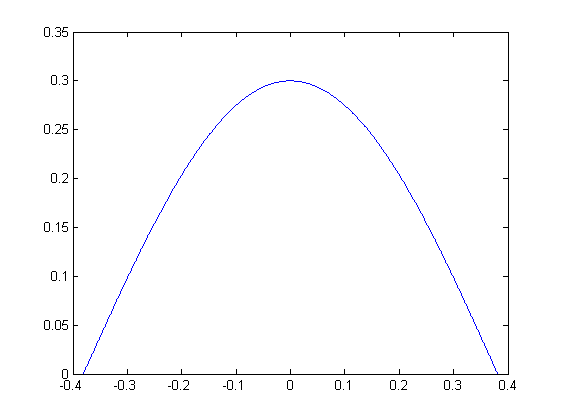
\includegraphics[width=\textwidth]{bow.png}

\section{Discussion}

While quite a few iterations are needed (around 1570) not a lot of calculations are done in each iteration. For each iteration we only calculate $a(q)$ and $arcLength(q, a)$. Thus the algorithm runs in $\mathcal{O}(n)$ and the execution time for our intital values is around 1 second. While the incrementation of $q$ (0.001) and the comparator for arc length (1e-5) are limiting factors for the precision of our output we do get close. Calculating y(q, x) with the values we found give us $1.836970198721030e-17$, which is fairly close to 0. See appendix A for implementation.

We did also implement an algorithm that uses the same assumptions and incrementation step for $q$ but instead of just calculating $a$ we used the matlab function ode45 (a solver for ordinary differential equations that uses an explicit Runge-Kutta method). This method would give us one x-value just before the function intersects the x-axis and one just below. Then using the secant method we could interpolate a more precise value for $a$ until either the arc length was close enough to 0.5 or it was time to pick a new $q$. Using this algorithm we did get an arc length of the same precision. However, calculating y(q, a) with these values gives us $-8.741237924993000e-03$, which is significantly less precise. While it did take fewer iterations (excluding the iterations done by ode45) it does take around 2 seconds to execute. See appendix B for implementation.

An algorithm I did not manage to implement properly was to use the upper and lower bounds of $a$ as start values for the secant method. However, the problem with that algorithm was to find a find a proper value for $q$ to calculate y(x). One solution was to perform the secant method for N steps before we increment $q$ by 0.001 but since we have the relationship $a(q)$ the secant method would be redundant.

\newpage
\appendix
\section{Final Implementation} \label{app:Appendix A}

\subsection{Main function}
\lstinputlisting{../test_bow.m}

\subsection{Function to calculate arc length}
\lstinputlisting{../arcLength.m}

\section{Alternative Implementation} \label{app:Appendix B}

\subsection{Main function}
\lstinputlisting{../old/hatarmittliv.m}

\subsection{Function to calculate the guesses for $a$}
\lstinputlisting{../old/guess_a.m}

\subsection{The given differential equation expressed a a set of low-order equations}
\lstinputlisting{../old/F2.m}

\subsection{Function to calculate arc length (same as other implementation)}
\lstinputlisting{../arcLength.m}

\end{document}
